\documentclass{article}


% if you need to pass options to natbib, use, e.g.:
%     \PassOptionsToPackage{numbers, compress}{natbib}
% before loading neurips_2023


% ready for submission
\usepackage{neurips_2024}


% to compile a preprint version, e.g., for submission to arXiv, add add the
% [preprint] option:
%     \usepackage[preprint]{neurips_2023}


% to compile a camera-ready version, add the [final] option, e.g.:
%     \usepackage[final]{neurips_2023}


% to avoid loading the natbib package, add option nonatbib:
%    \usepackage[nonatbib]{neurips_2023}


\usepackage[utf8]{inputenc} % allow utf-8 input
\usepackage[T1]{fontenc}    % use 8-bit T1 fonts
\usepackage{hyperref}       % hyperlinks
\usepackage{url}            % simple URL typesetting
\usepackage{booktabs}       % professional-quality tables
\usepackage{amsfonts}       % blackboard math symbols
\usepackage{nicefrac}       % compact symbols for 1/2, etc.
\usepackage{microtype}      % microtypography
\usepackage{xcolor}         % colors
\usepackage{graphicx}
\usepackage{amsmath}
\usepackage{mathtools}

\title{Uncertainty-Aware Super-Resolution Microscopy by Guided Diffusion}


% The \author macro works with any number of authors. There are two commands
% used to separate the names and addresses of multiple authors: \And and \AND.
%
% Using \And between authors leaves it to LaTeX to determine where to break the
% lines. Using \AND forces a line break at that point. So, if LaTeX puts 3 of 4
% authors names on the first line, and the last on the second line, try using
% \AND instead of \And before the third author name.


\author{%
  David S.~Hippocampus\thanks{Use footnote for providing further information
    about author (webpage, alternative address)---\emph{not} for acknowledging
    funding agencies.} \\
  Department of Computer Science\\
  Cranberry-Lemon University\\
  Pittsburgh, PA 15213 \\
  \texttt{hippo@cs.cranberry-lemon.edu} \\
  % examples of more authors
  % \And
  % Coauthor \\
  % Affiliation \\
  % Address \\
  % \texttt{email} \\
  % \AND
  % Coauthor \\
  % Affiliation \\
  % Address \\
  % \texttt{email} \\
  % \And
  % Coauthor \\
  % Affiliation \\
  % Address \\
  % \texttt{email} \\
  % \And
  % Coauthor \\
  % Affiliation \\
  % Address \\
  % \texttt{email} \\
}


\begin{document}


\maketitle


\begin{abstract}

Deep learning has recently attracted considerable attention from researchers in the natural sciences, particularly microscopists, for fast extraction of physically relevant information from images. In particular, single molecule localization microscopy has benefited significantly from recently developed deep kernel density estimators (KDE). However, simple and interpretable uncertainty quantification is lacking in these applications, and remains a necessary modeling component in high-risk research. In order to quantify uncertainty in otherwise deterministic image translation architectures, we propose a generative modeling framework based on denoising diffusion probabilistic models (DDPMs). Our model is inspired by guided diffusion, which condition the diffusion process with external cues or their derivatives. We propose uncertainty estimation by using a guided diffusion process to target diffusion toward a space of reasonable solutions through conditioning the score-estimator on a strong initial guess. This approach allows us to probe the structure of the distribution on reconstructions and estimate uncertainties. Our model is tested on KDE estimation in fluorescence microscopy, and we demonstrate that blending the traditional architectures with a DDPM permits simultaneous high-fidelity super-resolution with uncertainty estimation of regressed KDEs. 
\end{abstract}

\section{Introduction}

Deep learning has attracted tremendous attention from researchers in the natural sciences, with several foundational applications arising in microscopy, e.g., (Weigert 2018; Falk 2019). Recently, the application of deep image translation in single-molecule localization microscopy (SMLM) has received considerable interest (Ouyang 2018; Nehme 2020; Speiser 2021). SMLM techniques are a mainstay of fluorescence microscopy and can be used to produce a pointillist representation of biomolecules in the cell at diffraction-unlimited precision (Rust 2006; Betzig 2006). In previous applications of deep models to localization microscopy, super-resolution images can be recovered from a sparse set of localizations with conditional generative adversarial networks (Ouyang 2018) or kernel density estimation can be performed using traditional convolutional networks (Nehme 2020; Speiser 2021). Here, we focus on the latter class of models which perform KDE estimation using neural networks. 

Inferences in SMLM, and other super-resolution image reconstruction tasks, are often made on a single measurement, and thus common measures of model performance are based on localization errors computed over ensembles of simulated images. Unfortunately, this choice precludes computation of uncertainty at test time under a fixed model. Yet, Bayesian probability theory offers us mathematically grounded tools to reason about model uncertainty, but these usually come with a prohibitive computational cost (Gal 2022). A few approaches to avoiding this intractiblity in deep models have been deterministic uncertainty quantification (Amersfoort 2020), ensembling (Lakshminarayanan et al., 2017) or Monte Carlo dropout (Gal and Ghahramani, 2016). Here, we choose to model a distribution on high-resolution KDE predictions conditioned on a low-resolution input using a denoising diffusion probabilistic model (DDPM) (Ho 2020; Song 2021), Such models are one class of \emph{score based generative models} which implicitly compute the score of the data distribution at each noise scale starting from pure noise (Song 2021). This approach has proven powerful for generative modeling of conditional image distributions; however, conditional diffusion can become trapped in local optima preventing the application of such models to uncertainty estimation.

In statistical physics, particularly simulation of complex molecular systems, sampling is constrained to a limited set of configurations. For this reason, sampling begins at a presumed global optimum, which is typically a configuration with minimal energy (Levitt 1983). Similar notions of constrained diffusion have been used in DDPMs to guide the process based on gradients of a classifier (Nichols 2021). Importantly, in the context of DDPMs, the forward process is ill defined for corruption of a target image to a estimated global optimum. We therefore propose a guided diffusion process which targets diffusion toward a space of reasonable solutions by conditioning the score-estimator on a strong initial guess. This approach allows us to probe the structure of the distribution of reconstructions, with fewer iterations than standard diffusion models. Indeed, the entropy of estimated reconstructions obtained from guided diffusion must upper bound the entropy of reconstructions obtained from low-resolution inputs. This technique could be readily integrated with existing localization performance measures to address both model accuracy on training data and precision on datasets produced by experiments. 

\section{Background}

\subsection{Image Likelihood and Localization Error}

The central objective of single molecule localization microscopy is to infer a set of molecular coordinates $\theta=(\theta_{x},\theta_{y})$ from measured low resolution images $\bold{x}$. The likelihood on a particular pixel $k$, i.e., $p(\bold{x}_k|\theta)$ is taken to be a convolution of Poisson and Gaussian distributions, due to shot noise $p(s_{k}) = \mathrm{Poisson}(\omega_{k})$ and sensor readout noise $p(\zeta_{k}) = \mathcal{N}(o_{k},w_{k}^{2})$ 

\begin{equation}
p(\bold{x}_{k}|\theta) = A\sum_{q=0}^{\infty} \frac{1}{q!}e^{-\omega_{k}}\omega_{k}^{q}\frac{1}{\sqrt{2\pi}\sigma_{k}}e^{-\frac{(\bold{x}_{k}-g_{k}q-o_{k})}{2\sigma_{k}^{2}}} \approx \mathrm{Poisson}(\omega_{k}')
\end{equation}


\begin{figure}
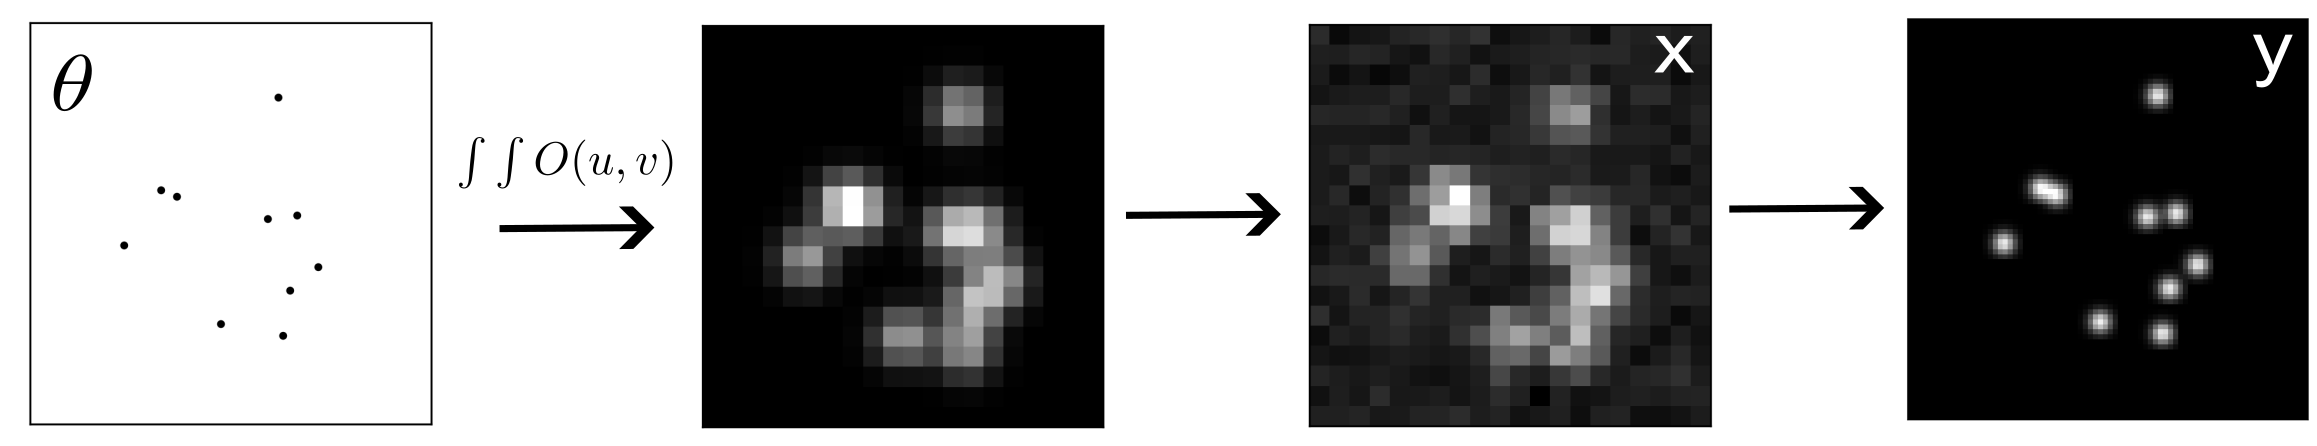
\includegraphics[scale=0.225]{Generation.png}
\caption{Generative model of single molecule localization microscopy images. Low resolution images $\bold{x}$ are generated from coordinates $\theta$ by integration of the optical transfer function $O$ and sampling from the likelihood (1): $\bold{x}\sim p(\bold{x}|\theta)$. A kernel density estimate $\bold{y}$ is inferred from $\bold{x}$}
\end{figure}

where $A$ is some normalization constant and $\omega_{k}' = \omega_{k} + w_{k}^{2}$. For the sake of generality, we include a per-pixel gain factor $g_{k}$, which is often unity. Sampling from $p(\bold{x}_{k})$ is trivial; however, for computation of a lower bound on uncertainty in $\theta$, the summation in (1) can be difficult to work with. Therefore, we choose to use a Poisson approximation for simplification, valid under a range of experimental conditions (Huang 2013). The expectation of the Poisson process at each pixel of the image must then be computed from the optical impulse response $O(u,v)$, which is taken to be an isotropic Gaussian in two-dimensions. For example, for a particular pixel of width $\delta$ located at $(u_k,v_k)$ in the first dimension

\begin{equation}
\Delta E_{\theta_{i}}(u_k,\theta_{x},\sigma_{\bold{x}}) \vcentcolon = \int_{u_{k}-\delta /2}^{u_{k}+\delta /2} O(\theta_{x})d\theta_{x} = \frac{1}{2}\left(\mathrm{erf}\left(\frac{u_{k}+\frac{1}{2}-\theta_{i}}{\sqrt{2}\sigma_{\bold{x}}}\right) -\mathrm{erf}\left(\frac{u_{k}-\frac{1}{2}-\theta_{i}}{\sqrt{2}\sigma_{\bold{x}}}\right)\right)
\end{equation}

The expected value at each pixel is then $\omega_{k}\propto \prod_{\theta_{i}\in (\theta_{x},\theta_{y})} \Delta E_{\theta_{i}}(\theta_{i},\sigma_{\bold{x}}) $. Using this, sampling from (1) is can be carried out by $\bold{x}_{k} = s_{k} + \zeta_{k}$ for $s_{k}\sim \mathrm{Poisson}(\omega_{k}), \eta_{k}\sim \mathcal{N}(o_{k},w_{k}^{2})$. The complete generative process is depicted in Figure 1. Reliable inference of $\theta$ from $\bold{x}$, for example by maximum likelihood estimation or with a deep model, requires performance metrics for model selection. We use the Fisher information as an information theoretic criteria to assess the quality of the model tested here, with respect to the root mean squared error (RMSE) of our predictions of $\theta$ (Chao 2016). The Poisson log-likelihood $\ell(\bold{x}|\theta)$ is also convenient for computing the Fisher information matrix (Smith 2010) and thus the Cramer-Rao lower bound, which bounds the variance of a statistical estimator of $\theta$, from below i.e., $\mathrm{var}(\hat{\theta}) \geq I^{-1}(\theta)$. The Fisher information is straightforward to compute under the Poisson log-likelihood, which is detailed in the Appendix

\begin{equation}
\mathcal{I}_{ij}(\theta) = \underset{\theta}{\mathbb{E}}\left(\frac{\partial \ell}{\partial\theta_{i}}\frac{\partial\ell}{\partial\theta_{j}}\right) = \sum_{k}\frac{1}{\omega_{k}'}\frac{\partial \omega_{k}'}{\partial\theta_{i}}\frac{\partial \omega_{k}'}{\partial\theta_{j}}
\end{equation}

\subsection{Gaussian kernel density estimation with deep networks}

Direct optimization of the likelihood in (1) from observations $\bold{x}$ alone is challenging when fluorescent emitters are dense within the field of view and fluorescent signals significantly overlap. However, convolutional neural networks (CNN) have recently proven to be powerful tools fluorescence microscopy to extract parameters describing fluorescent emitters such as color, emitter orientation, $z$-coordinate, and background signal (Zhang 2018; Kim 2019; Zelger 2018). For localization tasks, CNNs typically employ upsampling layers to reconstruct Bernoulli probabilities of emitter occupancy (Speiser 2021) or kernel density estimates with higher resolution than experimental measurements (Nehme 2020). We choose to use kernel density estimates in our model, denoted by $\bold{y}$. KDEs are the most common data structure used in SMLM, and can be easily generated from molecular coordinates, alongside observations $\bold{x}$, using well-understood models of the optical impulse response (Zhang 2007). 

\begin{figure}
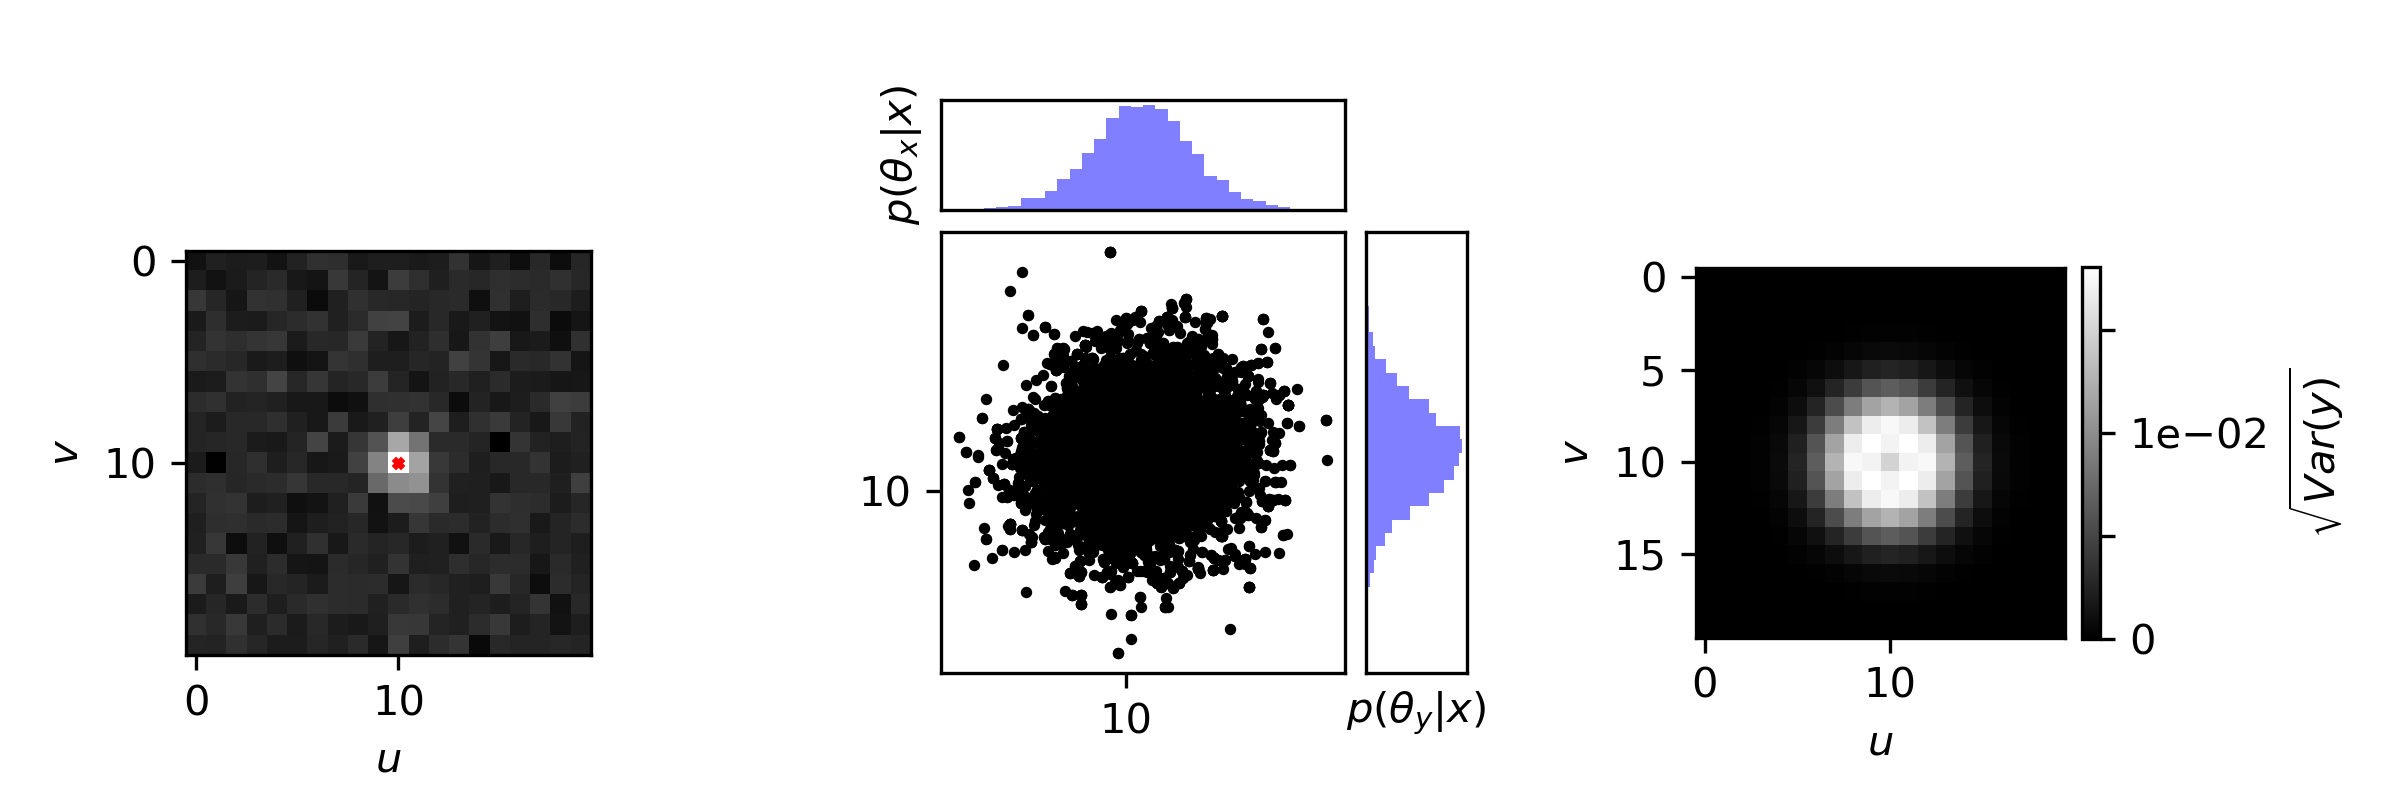
\includegraphics[scale=0.7]{MCMC.png}
\caption{Estimation of $\sqrt{\mathrm{Var}(\bold{y})}$ for in isolated fluorescent emitter.}
\end{figure}

Similar to the generative process on low resolution images $\bold{x}$, we can generate KDEs $\bold{y}$ by repurposing the generative model (1) on an unsampled image without noise. In other words, we cast Gaussian kernel density estimation as a noiseless image generation process on the domain of $\bold{y}$. Under a fixed configuration of $N$ particles $\theta$, the value of a KDE pixel $\bold{y}_{k}$ is given by

\begin{equation}
\bold{y}_{k}(\theta) = \sum_{n=1}^{N}\Delta E_{\theta_x}(u_{k},\theta_{n,x},\sigma_{\bold{y}}) \Delta E_{\theta_y}(v_{k},\theta_{n,y},\sigma_{\bold{y}})
\end{equation}

where the hyperparameter $\sigma_{\bold{y}}$ is the Gaussian kernel width. In principle, distribution on $\bold{y}_{k}$ is given directly from $p(\theta|\bold{x})$, which can be estimated by Metropolis-Hastings MCMC (Figure 2). For simplicity, in all following analysis, we are interested in the marginal variance $\mathrm{Var} (\bold{y}(\theta))$

\begin{equation}
\bar{\bold{y}}(\theta) = \underset{\theta\sim p(\theta|\bold{x})}{\mathbb{E}}\left[ \bold{y}(\theta)\right] \quad \mathrm{Var} (\bold{y}(\theta)) = \underset{\theta\sim p(\theta|\bold{x})}{\mathbb{E}}\left[ \bold{y}(\theta)-\bar{\bold{y}}(\theta)\right]^2
\end{equation}

Unfortunately, the posterior $p(\theta|\bold{x})$ can be costly to compute with MCMC, and is intractable at high molecular densities, as molecules cannot be easily resolved at test time. The central goal of this paper is to instead leverage a DDPM to model $p(\bold{y}|\bold{x})$, avoiding $p(\theta|\bold{x})$ entirely.

\section{Uncertainty-Aware Super-Resolution Microscopy by Guided Diffusion}

We consider datasets $(\bold{x}_i,\bold{y}_i,\hat{\bold{y}}_{i})_{i=1}^{N}$ of observed images $\bold{x}_i$ true kernel density estimate (KDE) images $\bold{y}_{i}$, and KDE estimates $\hat{\bold{y}}_{i}=\phi(\bold{x}_{i})$. Observations $\bold{x}_i$ are simulated under the convolution distribution (1) and KDEs are generated by (4).

\subsection{Problem Statement}

Point estimates $\hat{\bold{y}}_{i}$ produced by the traditional deep architectures for super resolution microscopy produce strong results, but lack uncertainty quantification. Recent advances in generative modeling, particularly DDPMs, therefore present a unique opportunity to integrate uncertainty awareness into the super-resolution microscopy toolkit. However, sampling from DDPMs is computationally expensive, given that generation amounts to solving a complex stochastic differential equation, effectively mapping a simple base distribution to the complex data distribution. The solution of such equations requires numerical integration with very small step sizes, resulting in thousands of neural network evaluations (Saharia 2021; Vahdat 2021). For conditional generation tasks in high-risk applications, generation complexity is further exacerbated by the need for the highest level of detail in generated samples. Moreover, in the present application, modeling the posterior is far more important than diversity in generated samples. Therefore, we propose that DDPM sampling is preceded by a deterministic neural network $\phi$, which effectively seeds sampling in a target mode. Reasoning for this choice in our application is two-fold:

\textbf{Synthesis Speed}. By training a preprocessor $\phi$ to obtain an approximate estimate of $\bold{y}$, we can reduce the number of iterations, since the DDPM only needs to model the remaining mismatch, resulting in a less complex model from which sampling becomes easier. Speed is critical in SMLM applications, which can produce thousands of images in a single experiment.\\

\textbf{Sample Fidelity}. Since Langevin dynamics will often be initialized in low-density regions of the data distribution, inaccurate score estimation in these regions will negatively affect the sampling process (Song 2019). Moreover, mixing can be difficult because of the need of traversing low density regions to transition between modes of the distribution. Preprocessing with a deterministic neural network $\phi$ can ameliorate this issue, by aiding score estimation in low density regions. 

Here, the model $\phi$ is realized by a CNN with upsampling layers. Consider the Markov chain wherein the KDE $\bold{y}$ is latent in and inferred from a noisy measurement $\bold{x}$, i.e., $\bold{x} \rightarrow \phi(\bold{x})\rightarrow \bold{\hat{y}}$. By the data processing inequality the function $\phi$ can only destroy information in $\bold{x}$ pertaining to $\bold{y}$ i.e., $I(\bold{x};\bold{y}) \geq I(\phi(\bold{x});\bold{y})$ or $h(\bold{y}|\phi(\bold{x})) \geq h(\bold{y}|\bold{x})$ where $I$ is the mutual information and $h$ is the entropy. This suggests that the uncertainty in $p_{\Psi}(\bold{y}|\phi(\bold{x}))$ is indeed an upper bound on the entropy of $p(\bold{y}|\bold{x})$. 

In practice, a DDPM $\Psi$ can be trained on pairs $(\bold{y}_i,\hat{\bold{y}}_{i})_{i=1}^{N}$. The conditional DDPM generates a target KDE $\bold{y}_0$ in $T$ refinement steps. Starting with a pure noise image $\bold{y}_{T}\sim \mathcal{N}(0,\bold{I})$, the model iteratively refines the KDE through successive iterations according to learned conditional transition distributions $p(\bold{y}_{t-1}|\bold{y}_{t},\bold{})$ such that $\bold{y}_{0} \sim p(\bold{y}|\hat{\bold{y}})$ 

\subsection{Guided Diffusion}

\begin{figure}
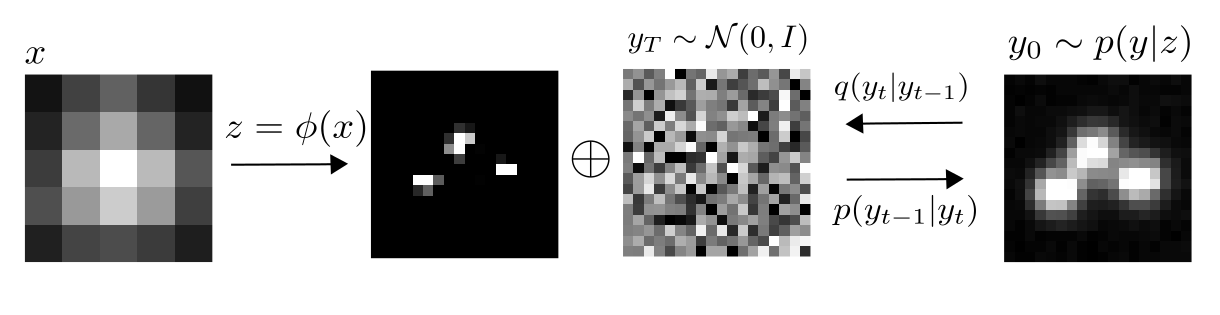
\includegraphics[scale=4.5]{Denoise.png}
\caption{Conditional diffusion model for sampling kernel density estimates}
\end{figure}

Diffusion models (Sohl-Dickstein 2015; Ho 2020; Song 2021) are a class of generative models inspired by nonequilibrium statistical physics, which slowly destroy structure in a data distribution $p(\bold{y}_{0}|\bold{x})$ via a fixed Markov chain referred to as the \emph{forward process}. In the present context, we apply leverage recent results from (Ho 2020; Song 2021; Saharia 2021) for applying this framework to sampling from $p(\bold{y}|\bold{x},\bold{\hat{y}})$. The forward process gradually adds Gaussian noise to the KDE $\bold{y}$ according to a variance schedule $\beta_{0:T}$

\begin{equation}
q(\bold{y}_{t}|\bold{y}_{0}) = \prod_{t=1}^{T}q(\bold{y}_{t}|\bold{y}_{t-1}) \;\;\; q(\bold{y}_{t}|\bold{y}_{t-1}) = \mathcal{N}\left(\sqrt{1-\beta_{t}}\bold{y}_{t-1},\beta_t I\right)
\end{equation}

The usual procedure is then to learn a parametric representation of the \emph{reverse process}, and therefore generate samples from  $p(\bold{y}_{0})$, starting from noise. Formally, $p_{\theta}(\bold{y}_{0}|\bold{\hat{y}}) = \int p_{\theta}(\bold{y}_{0:T}|\bold{\hat{y}})d\bold{\hat{y}}_{1:T}$ where $\bold{y}_{t}$ is a latent representation with the same dimensionality of the data.  $p_{\theta}(\bold{y}_{0:T}|\bold{\hat{y}})$ is a Markov process, starting from a noise sample $p_{\theta}(\bold{y}_{T}) = \mathcal{N}(0,\bold{I})$. 

\begin{equation}
p_{\theta}(\bold{y}_{0:T}) = p_{\theta}(\bold{y}_{T})\prod_{t=1}^{T} p_{\theta}(\bold{y}_{t-1}|\bold{y}_{t}) \;\;\; p_{\theta}(\bold{y}_{t-1}|\bold{y}_{t}) = \mathcal{N}\left(s_{\theta}(\bold{y}_{t}),\beta_{t}I\right)
\end{equation}

where we reuse the variance schedule of the forward process (Ho 2020). We omit conditioning on $\hat{\bold{y}}$ for each transition density $p_{\theta}(\bold{y}_{t-1}|\bold{y}_{t})$, as this is only considered at $t=0$ i.e., $p_{\theta}(\bold{y}_{1}|\bold{y}_{0},\hat{\bold{y}})$. An important property of the forward process is that it admits sampling $\bold{y}_t$ at an arbitrary timestep $t$ in closed form (Ho 2020). Using the notation $\alpha_t := 1 - \beta_t$ and $\gamma_t := \prod_{s=1}^{t} \alpha_s$, we have $q(\bold{y}_t|\bold{y}_0) = \mathcal{N} \left(\sqrt{\gamma_{t}} \bold{y}_{0}, (1 - \gamma_t)I \right)$.

\begin{equation}
\mathcal{L}(\theta) = \mathbb{E}\left[-\log p_{\theta}(\bold{y}_{0}|\bold{x})\right] \leq  \mathbb{E}\left[-\log \frac{p_{\theta}(\bold{y}_{0:T}|\bold{x})}{q(\bold{y}_{1:T}|\bold{y}_{0})}\right]
\end{equation}

The objective in (6) can be expanded in terms of $D_{\mathrm{KL}}(p(\bold{y}_{t-1}|\bold{y}_{t})|| q(\bold{y}_{t}|\bold{y}_{t-1})$ as detailed in (Ho 2020). We choose to adopt the simplified from of the variational bound, which is a reweighted form of the variational lower bound and emphasizes that the DDPM estimates the score $\nabla_{\bold{y}}\log p(\bold{y}|\bold{x})$ at each noise level (Song 2021)

\begin{equation}
\theta^{*} = \underset{\theta}{\mathrm{argmin}} \underset{(\bold{\hat{y}},\bold{y}_{0})}{\mathbb{E}}\underset{(\epsilon,\gamma)}{\mathbb{E}} \left[ s_{\theta}\left(x, \sqrt{\gamma} \bold{y}_0 + \sqrt{1 - \gamma} \epsilon \, \middle|\, \bold{y}_{t}, \gamma\right) - \epsilon \right],
\end{equation}

After training, samples can be generated by 

\begin{equation}
\bold{y}_{t-1} = \frac{1}{\sqrt{1-\beta_{i}}}\left(\bold{y}_{i} + \beta_{i}s_{\theta}(\bold{y}_{t})\right) + \sqrt{\beta_{i}}\bold{\xi}
\end{equation}


\section{Experiments}

\begin{figure}
\centering
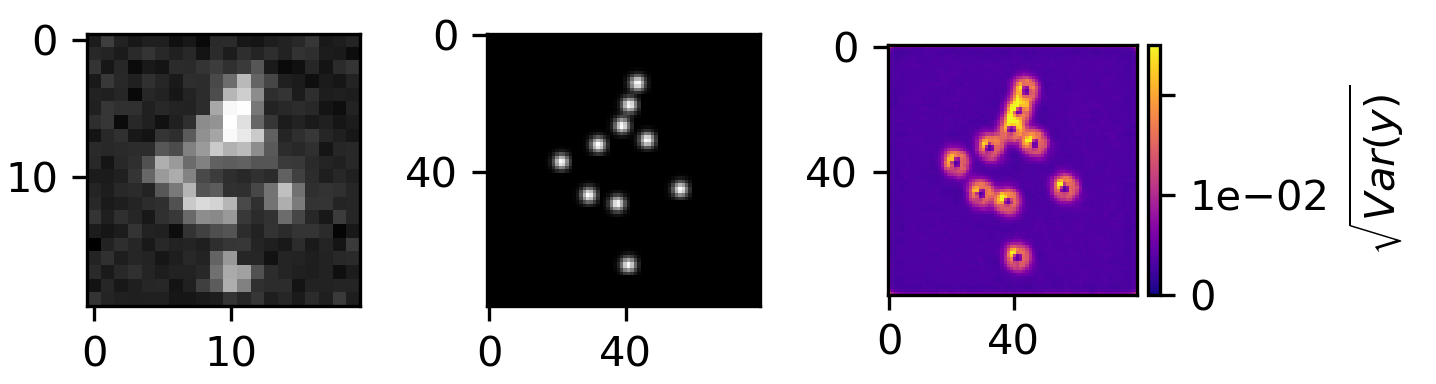
\includegraphics[scale=1.2]{Bayes.png}
\caption{Kernel density estimates for various signal to noise ratios (SNR)}
\end{figure}

All training data consits of low-resolution $20\times 20$ images, simulated as described previously, setting $\sigma_{\bold{x}}=0.92$ in units of low-resolution pixels, for consistency with common experimental conditions with a 60X magnification objective lens and numerical aperture (NA) of 1.4. We choose $i_{0}=200$ for experiments for consistency with typical bright fluorophore emission rates. All KDEs have dimension $80\times 80$, are scaled between $[0,1]$, and are generated using $\sigma_{\bold{y}}=3.0$ pixels in the upsampled image. For a typical CMOS camera, this results in KDE pixels with lateral dimension of $\approx 27\mathrm{nm}$. Initial coordinates $\theta$ were drawn uniformly over a two-dimensional disc with a radius of 7 low-resolution pixels.

\subsection{Localization RMSE}

In order to verify the initial predictions made by the model $\phi$, we simulated a dataset $(\bold{x}_i,\bold{y}_i,\hat{\bold{y}}_{i})_{i=1}^{N}$ with $N=1000$, and  detect objects in the predicted KDE $,\hat{\bold{y}}_{i}$ using the Laplacian of Gaussian (LoG) detection algorithm (Lindeberg 2013). Localization is carried out from scale-space maxima directly in LoG, as opposed to fitting a model function to KDE predictions. A particular LoG localization in the KDE is paired to the nearest ground truth localization and is unpaired if a localization is not within 5 KDE pixels of any ground truth localization. In addition to localization error, we measure a precision $\mathrm{P = TP/(TP + FP)} = 1.0$ and recall $\mathrm{R = TP/(TP + FN)} = 0.85$, where $\mathrm{TP}$ denotes true positive localizations, $\mathrm{FP}$ denotes false positive localizations, and $\mathrm{FN}$ denotes false negative localizations.

\subsection{Guided Diffusion}

We set $T = 100$ for all experiments and treat forward process variances $\beta_{t}$ as hyperparameters, with a linear schedule from $\beta_{0}=10^{-4}$ to $\beta_{T}=10^{-2}$.
These constants were chosen to be small relative to ground truth KDEs, which are scaled to $[-1,1]$, ensuring that forward process distribution $\bold{y}_{T}\sim q(\bold{y}_{T}|\bold{y}_{0})$ approximately matches the reverse process $\bold{y}_T\sim \mathcal{N}(0, I)$ at $t=T$.

To represent the reverse process, we used a DDPM architecture based on a U-Net backbone proposed in (Saharia 2021). We chose a U-Net backbone with channel multipliers $[1,2,4,8,8]$ in the downsampling and upsampling paths of the architecture. Parameters are shared across time, which is specified to the network using the Transformer sinusoidal position embedding. We use self-attention at the $16 \times 16$ feature map resolution. To condition the model on the input $\bold{\hat{y}}$, we concatenate the $\bold{\hat{y}}$ estimated by DeepSTORM along the channel dimension, which are scaled to $[0,1]$, with $\bold{y}_T\sim \mathcal{N}(0, I)$. Others have experimented with more sophisticated methods of conditioning, but found that the simple concatenation yielded similar generation quality (Saharia 2021). 


\section{Conclusion}


\clearpage
\section*{References}


{
\small


[1] Nehme, E., et al. DeepSTORM3D: dense 3D localization microscopy and PSF design by deep learning. Nature Methods 17, 734–740 (2020).


[2] Ouyang, W., et al. Deep learning massively accelerates super-resolution localization microscopy. Nature Biotechnology 36, 460–468 (2018).


[3] Speiser, A., et al. Deep learning enables fast and dense single-molecule localization with high accuracy. Nature Methods 18, 1082–1090 (2021).

[4] Sohl-Dickstein J., et al. Deep unsupervised learning using nonequilibrium thermodynamics. ICLR (2015).

[5] Ho J., et al. Denoising Diffusion Probabilistic Models. Advances in Neural Information Processing Systems (2015).

[6] Nanxin C., et al. WaveGrad: Estimating Gradients for Waveform Generation
. ICLR (2021).

[4] Chao, J., et al. Fisher information theory for parameter estimation in single molecule microscopy: tutorial. Journal of the Optical Society of America A 33, B36 (2016). 

[5] Schermelleh, L. et al. Super-resolution microscopy demystified. Nature Cell Biology vol. 21 72–84 (2019). 

[6] Zhang, B., et al. Gaussian approximations of fluorescence microscope point-spread function models. (2007). 

[7] Smith, C.S.,  Fast, single-molecule localization that achieves theoretically minimum uncertainty. Nature Methods 7, 373–375 (2010). 

[8] Nieuwenhuizen, R., et al. Measuring image resolution in optical nanoscopy. Nature Methods 10. 557-562 (2013). 

[9] Huang, F., et al. Video-rate nanoscopy using sCMOS camera-specific single-molecule localization algorithms. Nat Methods 10, 653–658 (2013). 

[10] Rust, M., et al. Sub-diffraction-limit imaging by stochastic optical reconstruction microscopy (STORM). Nat Methods 3, 793–796 (2006).

[11] Betzig, E., et al. Imaging intracellular fluorescent proteins at nanometer resolution. Science 313, 1642–1645 (2006).

[12] Weigert, M., et al. Content-aware image restoration: pushing the limits of fluorescence microscopy. Nat. Methods 15, 1090 (2018).

[13] Falk, T., et al. U-net: deep learning for cell counting, detection, and morphometry. Nat. Methods 16, 67–70 (2019).

[14] Boyd, N., et al. DeepLoco: fast 3D localization microscopy using neural networks. Preprint at bioRxiv https://doi.org/10.1101/267096 (2018)

[15] Zelger, P., et al. Three-dimensional localization microscopy using deep learning. Opt. Express 26, 33166–33179 (2018)

[16] Zhang, P., et al. Analyzing complex single-molecule emission patterns with deep learning. Nat. Methods 15, 913 (2018)

[17] Saharia, C., et al. Image Super-Resolution via Iterative Refinement. Preprint at arXiv https://doi.org/10.48550/arXiv.2104.07636 (2021)

[18] Kim, T., et al. Information-rich localization microscopy through machine learning. Nat Commun 10, 1996 (2019). 

}

\appendix

\section{Appendix}

\subsection{Optical impulse response}

It is common to describe the optical impulse response of a microscope as a two-dimensional isotropic Gaussian (Zhang 2007). This is an approximation to the more rigorous diffraction models given by Richards and Wolf (1959) or Gibson and Lanni (1989). Over a continuous domain, the impulse response reads

\begin{equation*}
\mathrm{G}(u,v) = \frac{1}{2\pi\sigma_{\bold{x}}^{2}}e^{-\frac{(u-\theta_{x})^{2}+(v-\theta_{y})^{2}}{2\sigma_{\bold{x}}^{2}}}
\end{equation*}

The above expression can be interpreted as a probability distribution over locations where a photon can be detected. Therefore, for discrete detectors, we discretize this expression by integrating over pixels. The number of photon arrivals will follow Poisson statistics, with expected value

\begin{equation}
\omega_{k} = i_{0}\left(\int_{u_{k}-\delta /2}^{u_{k}+\delta /2} O(\theta_{x})d\theta_{x} \right)\left(\int_{v_{k}-\delta /2}^{v_{k}+\delta /2} O(\theta_{y})d\theta_{y} \right)
\end{equation}

The scalar quantity $i_{0}$ represents the amplitude of the signal, which is proportional the quantum efficiency of a pixel $\eta$, the duration of exposure, $\Delta$, and the number of photons emitter by a fluorescent molecule $N_{0}$. With no loss of generality, $\Delta = \eta = 1$ and there is a single free parameter $N_{0}$. Furthermore, to simplify the notation, in the main text we define

\begin{equation}
\Delta E_{\theta_{i}}(u_k,\theta_{x},\sigma_{\bold{x}}) \vcentcolon = \int_{u_{k}-\delta /2}^{u_{k}+\delta /2} O(\theta_{x})d\theta_{x} = \frac{1}{2}\left(\mathrm{erf}\left(\frac{u_{k}+\frac{1}{2}-\theta_{i}}{\sqrt{2}\sigma_{\bold{x}}}\right) -\mathrm{erf}\left(\frac{u_{k}-\frac{1}{2}-\theta_{i}}{\sqrt{2}\sigma_{\bold{x}}}\right)\right)
\end{equation}

where we have used the common definition $\mathrm{erf}(z) = \frac{2}{\sqrt{\pi}}\int_{0}^{t}e^{-t^{2}}dt$. 

\subsection{Metropolis-Hastings MCMC}

To obtain numerical estimates of $p(\theta|\bold{x}\propto p(\bold{x}|\theta)p(\theta)$ and therefore $p(\bold{y}|\bold{x})$, for an isolated fluorescent molecule as shown in (Figure 2), we used Metropolis-Hastings Markov Chain Monte Carlo (MCMC) to estimate the posterior marginals on coordinates. Under the Poisson approximation in (1), the model negative log-likelihood is

\begin{equation}
\ell(\bold{x}|\theta) = -\log \prod_{k} \frac{e^{-\left(\omega_{k}'\right)}\left(\omega_{k}'\right)^{n_{k}}}{n_{k}!} = \sum_{k}  \log n_{k}! + \omega_{k}' - n_{k}\log\left(\omega_{k}'\right)
\end{equation}

MCMC is asymptotically exact, which is not guaranteed by variational methods which may rely on a Laplace approximation around the MLE. We choose a uniform prior $p(\theta)$, and Metropolis-Hastings is run for $10^4$ iterations, the first $10^{3}$ iterations is discarded as burn-in. A proposal $\theta' = \theta + \xi$ was generated with $\xi\sim \mathcal{N}(0,\sigma^{2}I)$ where $\sigma^{2}=0.05$. The acceptance probability is

\begin{equation*}
\alpha = e^{\beta(\ell(\theta)-\ell(\theta'))}
\end{equation*}

We choose $\beta=0.2$ to achieve a target acceptance rate of $0.5$.

\subsection{Cramer-Rao Lower Bound}

The Poisson approximation is also convenient for computing the Fisher information matrix for $\theta_{\mathrm{MLE}}$ and thus the Cramer-Rao lower bound, which bounds the variance of a statistical estimator of $\theta_{\mathrm{MLE}}$, from below (Chao 2016). The Fisher information is

\begin{equation}
I_{ij}(\theta) = \underset{\theta}{\mathbb{E}}\left(\frac{\partial \ell}{\partial\theta_{i}}\frac{\partial\ell}{\partial\theta_{j}}\right) 
\end{equation}

Let $\mu_{k}' = g_{k}\mu_{k} + \sigma_{k}^{2}$. For an arbitrary parameter,

\begin{align*}
\frac{\partial \ell}{\partial \theta_{i}} &= \frac{\partial}{\partial \theta_{i}} \sum_{k}  x_{k}\log x_{k} + \mu_{k}' - x_{k}\log\left(\mu_{k}'\right)\\
&= \sum_{k} \frac{\partial \mu_{k}'}{\partial\theta_{i}} \left(\frac{\mu_{k}'-x_{k}}{\mu_{k}'}\right)
\end{align*}

\begin{equation*}
I_{ij}(\theta) = \underset{\theta}{\mathbb{E}}\left(\sum_{k}\frac{\partial \mu_{k}'}{\partial\theta_{i}}\frac{\partial \mu_{k}'}{\partial\theta_{j}} \left(\frac{\mu_{k}'-x_{k}}{\mu_{k}'}\right)^{2}\right) = \sum_{k}\frac{1}{\mu_{k}'}\frac{\partial \mu_{k}'}{\partial\theta_{i}}\frac{\partial \mu_{k}'}{\partial\theta_{j}}
\end{equation*}

\begin{figure}
\centering
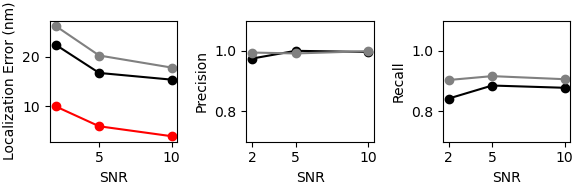
\includegraphics[scale=0.7]{Errors.png}
\caption{Localization errors of the trained model}
\end{figure}


\subsection{DeepSTORM CNN}

The DeepSTORM CNN, initially proposed in (Nehme 2020) for 3D localization, can be viewed as a deep kernel density estimator, reconstructing kernel density estimates $\bold{y}$ from low-resolution inputs $\bold{x}$. We utilize a simplified form of the original architecture for 2D localization, which we denote $\phi$ hereafter, which consists of three main modules: a multi-scale context aggregation module, an upsampling module, and a prediction module. For context aggregation, the architecture utilizes dilated convolutions to increase the receptive field of each layer. The upsampling module is then composed of two consecutive 2x resize-convolutions, computed by nearest-neighbor interpolation, to increase the lateral resolution by a factor of 4. For a common sCMOS camera, each pixel has a lateral size of approximately 108 nanometers, giving approximately 27 nanometer pixels in the KDE. The terminal prediction module contains three additional convolutional blocks for refinement of the upsampled image, followed by an element-wise HardTanh. 



\end{document}
